\graphicspath{{04-KL/Figures/}}

\section{KLOE-Light Calorimeter}
\label{Sect:KL}

\subsection{Introduction}
\label{SubSect:KL_Intro}
% v2 - Domizia Orestano reviewed this (Ludovico Tortora and Mariyan Bogomilov in cc)

The KLOE-Light (KL) pre-shower sampling calorimeter is composed of extruded lead foils in which scintillating
fibres are placed in volume ratio scintillator:lead~$\sim$~2:1, ``lighter'' than the one of the KLOE experiment calorimeter~(1:1).

The fibres are 1~mm diameter BICRON BCF-12, scintillating in the blue, 1.35~mm distant from each other within a layer. The distance between two layers is 0.98~mm, one layer being shifted by half the fibre pitch with respect to the next.
Scintillation light is guided from each slab into a total of six PMTs (three on each side). Iron shields are fitted to each photomultiplier to
mitigate against large stray magnetic fields from the cooling channel (see~Fig.~\ref{fig:KL1}). The signal from each PMT is sent to a shaping amplifier (SA) module, which shapes and stretches the signal in time in order to match the sampling rate of the flash ADCs (Fig.~\ref{fig:KL2} shows the design of a single slab).
A total of 7 slabs forms the whole detector, which has an active volume of 93~cm$\times$93~cm$\times$4~cm.

With its 2.5 radiation lengths the KL is used to distinguish muons from decay electrons providing energy deposition and timing information and to act as pre-shower in front of the EMR.
The detector has been used to estimate the level of pion contamination within the MICE muon beams to be around~1\%~\cite{2016JInst..11P3001A}.
\begin{figure}
  \begin{center}
    \includegraphics[width=0.4\columnwidth]{./04-KL/Figures/KL1.png}
    \caption{Magnetic shielding of KLOE-Light PMTs.}
    \label{fig:KL1}
  \end{center}
\end{figure}
\begin{figure}
  \begin{center}
    \includegraphics[width=0.8\columnwidth]{./04-KL/Figures/KL2.png}
    \caption{Single slab design of MICE KLOE-Light Calorimeter.}
    \label{fig:KL2}
  \end{center}
\end{figure}



\subsection{Performance}
\label{SubSect:KL_Performance}

The study of KL response to different particle types at different momenta is based on particle identification obtained by time-of-flight detector, as shown in the example of~Fig.~\ref{fig:TOF_peaks}, by applying proper cuts on the time-of-flight spectrum. The performance is presented for 140, 170, 200, 240 and 300 MeV/c momenta at the absorber position, and depending of species population for muons, pions and electrons. The results presented below are obtained from the straight tracks data (i.e. without magnetic fields in the trackers or focus coil) taken mainly in 2017. The KL response to muons, pions and electrons for all available momenta is presented in~Fig.~\ref{fig:KL_to_mu_pi_e}. It is clear in the cases of muons and pions that they are below mip momenta since energy deposition decreases with momentum increasing~\footnote{Actually the energy deposition is defined as the sum of ADC products from all cells in KL above a given threshold. The ADC product on the other hand is the product of left and right side of one slab divided by the sum of left and right side: $ADC_{prod} = 2 \times ADC_{left}  \times ADC_{right} / (ADC_{left} + ADC_{right})$. The factor 2 is present for normalization. The product of two sides compensates the effect of attenuation.}.
  \begin{figure}
	\begin{center}
  		\includegraphics[width=0.3\columnwidth]{./04-KL/Figures/muon.png}
  		\includegraphics[width=0.3\columnwidth]{./04-KL/Figures/pion.png}
  		\includegraphics[width=0.3\columnwidth]{./04-KL/Figures/electron.png}
  		\caption{KL response to muons (left), pions (centre) and electrons (right) for several momenta. It is shown charge deposited by particles in KL in arbitrary units. All histograms are normalized to unity.}
  		\label{fig:KL_to_mu_pi_e}
  	\end{center}
  \end{figure}

For comparison of energy deposition of muon, pions and electrons for fixed momentum~Fig.~\ref{fig:KL_mu_to_pi} is presented. In the case of 300 MeV/c (~Fig.~\ref{fig:KL_mu_to_pi}, right), where muons and pions have almost the same maximum of distribution, the tail of pions is fatter than muon one. This is due to the fact that pions experience strong interaction as well. This pion behaviour has been used to estimate its contamination in muon sample. 

The number of fired KL cells by a single muon, electron or pion is given in ~Fig.~\ref{fig:KL_mult} for 240 MeV/c beam. For muons we expect one, in some cases two and almost never more fired cells depending on track inclination. Pions and electrons create avalanches in KL and electron ones is much wider than the pion ones as visible of number of KL cell hits. The same figure shows number of events when if there is a reconstructed TOF track, but no signal in KL above the threshold. This can be used to calculate efficiency of KL for the three species as a function of momentum. The results are presented in ~Table~\ref{tab:KL_eff} and shows that efficiency for muon registration is close to 99$\%$.


 

   \begin{figure}
   	\begin{center}
   		\includegraphics[width=0.4\columnwidth]{./04-KL/Figures/mu_vs_pi_vs_e_200MEV.png}  		\includegraphics[width=0.4\columnwidth]{./04-KL/Figures/mu_vs_pi_300MEV.png}
   		\caption{Comparison of energy deposition of muons, pions and electrons at 200 MeV/c (left) and of muons to pions at 300 MeV/c (right).}
   		\label{fig:KL_mu_to_pi}
   	\end{center}
   \end{figure}
    \begin{figure}
    	\begin{center}
    		\includegraphics[width=0.4\columnwidth]{./04-KL/Figures/multiplicity_240MEV.png}  		
    		\caption{Particle multiplicity for 240 MeV/c, i.e. number of KL cells fired.}
    		\label{fig:KL_mult}
    	\end{center}
    \end{figure}
       
  \begin{table}[htb]
  	\begin{center}
  		\begin{tabular}{|c|c|c|c|c|c|} 
  			\hline
  			\textbf{species} &\textbf{140 MeV/c} & \textbf{170 MeV/c} & \textbf{200 MeV/c}	&\textbf{240 MeV/c} &\textbf{300 MeV/c}\\
  			\hline
  			\textbf{electrons} & 0.95 $\pm$ 0.02  & 0.95 $\pm$ 0.01 & 0.94 $\pm$ 0.03 & n/a & n/a \\
  			\hline
  			\textbf{muons} &  0.97$\pm$ 0.02 & 0.99 $\pm$ 0.01  & 0.99 $\pm$  0.01 & 0.99 $\pm$ 0.01 & 0.99$\pm$ 0.01\\
  			\hline
  			\textbf{pions} &  n/a  & 0.89 $\pm$ 0.03  & 0.95 $\pm$ 0.03 & 0.97 $\pm$ 0.03 & 0.98$\pm$ 0.01\\
  			\hline
  		\end{tabular}
  		\caption{Efficiency of KL for electrons, muons and pions as a function of particle momentum. The conditions required are existing of a TOF track and signal in KL above the threshold. The uncertainties are statistical.}
  		\label{tab:KL_eff}
  	\end{center}
  \end{table}

In~Fig.~\ref{fig:KL_mc_vs_data} is shown simulation of KL response to 300 MeV/c muons and pions and the distributions are compared with data. The agreement between data and simulation is very good. The simulation is done via following steps:

\begin{itemize}
	\item Smearing of produced photons in scintillator fibres. They obtain Poisson statistic so such is applied. In principal one can replace it with Gaussian because the number of photons created is  large enough for such an approximation.
	
	\item Photoelectrons created on photomultiplier photocathode also have Poisson statistics. It cannot be replaced here with normal distribution because the number of photoelectrons is small enough so such an approximation is illegal.
	
	\item Photomultiplier gain obtains also statistical properties but it is neither Poisson nor gauss. Nevertheless it turns out that for simplicity one can use Gaussian distribution with mean value equals to PMT gain and sigma of distribution equals to half of the gain. KL photomultipliers have gain $\sim 2 \times 10^6$, so their sigma is simply $10^6$.
	
\end{itemize}

   \begin{figure}
   	\begin{center}
   		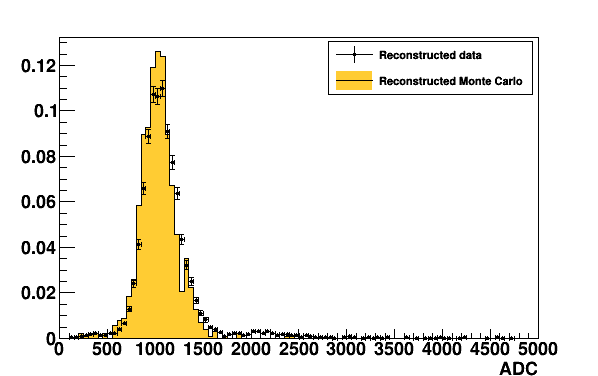
\includegraphics[width=0.4\columnwidth]{./04-KL/Figures/muon_mc_vs_data.png}  		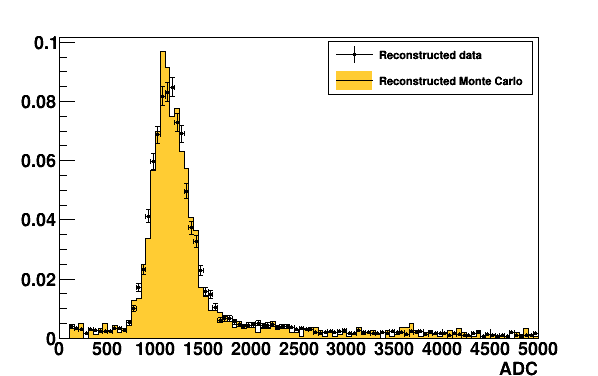
\includegraphics[width=0.4\columnwidth]{./04-KL/Figures/pion_mc_vs_data.png}
   		\caption{Comparison between data and Monte Carlo simulation of KL response to muons (left) and pions (right) at 300 MeV/c.}
   		\label{fig:KL_mc_vs_data}
   	\end{center}
   \end{figure}
